\documentclass{standalone}

\usepackage{tikz}
\usepackage{tkz-euclide}
\usetikzlibrary{calc}
\usetikzlibrary{positioning}
\usetikzlibrary{arrows.meta}

\usepackage{times}


\begin{document}
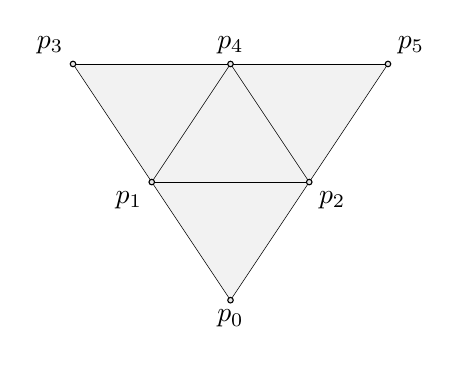
\begin{tikzpicture}[%
  >={Stealth[scale=1.0]},
  scale=1.0,
]

  \tkzDefPoint(0.0, 0.0){v0}
  \tkzDefPoint(2.0, 0.0){v1}
  \tkzDefPoint(1.0, 1.5){v2}
  \tkzDefPoint(1.0, -1.5){v3}
  \tkzDefPoint(3.0, 1.5){v4}
  \tkzDefPoint(-1.0, 1.5){v5}

  \tkzFillPolygon[color=black!5](v0,v1,v2)
  \tkzFillPolygon[color=black!5](v0,v1,v3)
  \tkzFillPolygon[color=black!5](v1,v2,v4)
  \tkzFillPolygon[color=black!5](v2,v0,v5)

  \tkzDrawSegments(v0,v1 v1,v2 v2,v0 v0,v3 v3,v1 v1,v4 v4,v2 v2,v5 v5,v0)

  \tkzDrawPoints(v0,v1,v2,v3,v4,v5)

  \tkzLabelPoint[below left](v0){$p_1$}
  \tkzLabelPoint[below right](v1){$p_2$}
  \tkzLabelPoint[above](v2){$p_4$}
  \tkzLabelPoint[below](v3){$p_0$}
  \tkzLabelPoint[above right](v4){$p_5$}
  \tkzLabelPoint[above left](v5){$p_3$}

\end{tikzpicture}
\end{document}
